\documentclass[12pt]{article}
\usepackage[a4paper, portrait, margin=1in]{geometry}
\usepackage{amsmath}
\usepackage{titling}
\usepackage{minted}
\usepackage{pgfplots}
\usepackage[none]{hyphenat}
\usepackage{graphicx}
\usepackage{wrapfig}
\usepackage[format=plain,
    font={small, it}, justification=centering]{caption}
\setkeys{Gin}{width=14cm}
\definecolor{bg}{rgb}{0.95,0.95,0.95}
\setminted{linenos=true, fontsize=\footnotesize, bgcolor = bg}
\usetikzlibrary{external}
\tikzexternalize[prefix=figures/]
\pgfplotsset{width=10cm, compat=1.18}
\DeclareMathOperator{\sinc}{sinc}

\author{
    Charlie Turner: n10752846
    \and
    Joel Kemp: n10746862
    \and
    Viet Truong Minh: n10440151
}
\title{EGB242 Assignment 2}

\begin{document}

\begin{titlingpage}
    \maketitle
\end{titlingpage}

\section*{Introduction}

After the chief at Brisbane-based Australian Space Agency (BASA) has reviewed
previous tasks, they have decided to assign the team `live' supervision of the
MARS-242 mission.

Communication between the ground and the mission must be clear and
uninterrupted to ensure the mission is safe and smooth. There are three
important tasks to be completed:
\begin{itemize}
    \item[-] Identifying an appropriate landing site for the crew
    \item[-] Ensuring the safety of the Martian habitats for the current and future crews
\end{itemize}

\noindent To achieve these objectives, the team must be able to properly interpret and
analyse data streams from a rover scouting the surface prior to landing.
The landing site must be identified despite periodic and bandlimited noise
disrupting signal streams. Once a landing site is determined, the acoustic
properties of the habitat's rooms must be analysed, removing interference and
noise arising from the communication channel and method.

%--------------------------------------------------------------------------
%
% SECTION 1: MARS ROVER
%
%--------------------------------------------------------------------------
\section{Mars Rover}

With the crew landing soon, a rover has been gathering data regarding possible
landing sites. Until a malfunction on the rover, data has been communicated
directly with Earth, where it can be analysed and the results sent directly to
astronauts on board Mars-242. The rover's data is vital for the survival of the
mission, so a solution has been found to send the raw data directly to
astronauts, but there are complications in this process.

\subsection*{Communication Channels}
\begin{math}
    s_{rov}(t) = 8000 \times \sinc^2(4000t)\cos(2\pi \times 8000t)
\end{math}
\subsection*{Rover Transmission Function}
\subsection*{Filtering Information}
\subsection*{Signal Recovery}
\pagebreak

%--------------------------------------------------------------------------
%
% ---------------------SECTION 2: LANDING SITE-----------------------------
%
%--------------------------------------------------------------------------
\section{Choosing a Landing Site}

The surface-based rover has collected and transmitted images of possible
landing sites. Unfortunately, the transmission encountered both periodic and
bandlimited noise, so the signals must be denoised to observe the intended
images. One of the noisy images is visualised in Fig.~\ref{fig:p2-noisy}. This
is achieved in MATLAB using the \verb+reshape+ function, reshaping the incoming
1D data stream into a matrix, knowing that the images are all of the same size
(640$\times$480).

\begin{figure}[ht]
    \centering
    \includegraphics[width=7cm]{figures/p2-noisy.png}
    \caption{Noisy image of possible landing site\label{fig:p2-noisy}}
\end{figure}

\subsection{Modelling Periodic Noise}

To understand the characteristics of relevant noise, the signal is plotted in
both the time and frequency domain as in Fig.~\ref{fig:p2-timefreq},
understanding the importance of the sampling rate for the incoming signal:
\begin{minted}{matlab}
Fs = 1000;                                  % Pixel Sampling Rate [Hz]
T = pixels/Fs;                              % Time to recieve an image
t = linspace(0, T, length(sig)+1);          % Time vector for full image
f = linspace(-Fs/2, Fs/2, length(sig)+1);   % Frequency Vector
\end{minted}

\begin{figure}[h]
    \centering
    \includegraphics{figures/p2-timefreq.png}
    \caption{Time and Frequency Domain of Incoming Signal\label{fig:p2-timefreq}}
\end{figure}

While the full signal for an image is over 300 seconds long, plotting only the
first three seconds shows that there is a significant periodic noise present in
the time domain. Engineers at mission control have identified a set of possible
periods for the noise, and graphically we can determine that it appears to be
approximately 1.477 seconds long, confirming the engineers approximations.
Using MATLAB and the provided \verb+estimateNoise+ function, a vector
representing one period of this noise was computed:
\begin{minted}[firstnumber=62]{matlab}
T = candidateT(1);                                       % 1.477s 
noisePeriodSamples = T * Fs;                             % samples in 1.477s 
Noisesig = estimateNoise(sig(1, :), noisePeriodSamples); % estimated noise 
\end{minted}

Comparing the estimated noise to the received signal in
Fig.~\ref{fig:p2-noisecomp}, we can see that the overall shape of the signals
is similar.

\begin{figure}[ht]
    \centering
    \includegraphics{figures/p2-noisecomp.png}
    \caption{Comparison of Estimated Noise and Recieved Signal\label{fig:p2-noisecomp}}
\end{figure}

With the correct discrete representation of periodic noise determined, we can
model \verb+Noisesig+ with a complex fourier series as follows:

\begin{align*}
    x(t)             & = \sum_{n=-\infty}^{\infty} c_n \exp(j 2\pi n f_0 t)        \\
    \text{with } c_n & = \frac{1}{T} \int^{t_0 + T}_{t_0} x(t)e^{-j2\pi nf_0 t} dt
\end{align*}

In MATLAB, integrals are substituted for Riemann sums on the discrete vector,
computing $c_n$ for $-6\le n \le 6$ taking into account an accurate time vector
and sampling rate:

\begin{minted}{matlab}
t1= t(t<T); t1(end) = [];                           % Noise Time vector 
ts = t1(2)-t1(1);                                   % Sampling interval [s]
f0 = 1/T;                                           % Fundamental Frequency
N = 6;                                              % Number of harmonics
n = (-N:N).';                                       % Vector of harmonics
cn = f0 * Noisesig * exp(-1j*2*pi*f0*n*t1).' * ts;  % Fourier coefficients
c0 = cn(N+1);                                       % DC coefficient
NoisesigApprox = cn * exp(1j*2*pi*n*f0*t1);         % Fourier approximation
\end{minted}

The DC coefficient is computed as $c_0 = +0.3571$, and the complex coefficients
for the first 6 harmonics as follows:
\[
    \begin{array}{ccc}
        c_{-6} : -0.2208 + 0.4813i & c_{-5} : +0.2479 - 0.2237i & c_{-4} : +0.0260 - 0.1276i \\
        c_{-3} : -0.4525 + 0.1048i & c_{-2} : -0.2916 + 0.2814i & c_{-1} : -0.3702 + 0.1522i \\
        c_{+1} : -0.3702 - 0.1522i & c_{+2} : -0.2916 - 0.2814i & c_{+3} : -0.4525 - 0.1048i \\
        c_{+4} : +0.0260 + 0.1276i & c_{+5} : +0.2479 + 0.2237i & c_{+6} : +0.2208 + 0.4813i \\
    \end{array}
\]

BASA has confirmed that there should be no DC component to the periodic noise.
Because $c_0$ represents the DC component of the Fourier series, this term can
simply be equated to 0 in order to remove this bias:

\begin{minted}[firstnumber=62]{matlab}
cn(N+1) = 0;                                   % remove DC bias
\end{minted}

With the correct Fourier coefficients determined, the signal can be
reconstructed for the total period of the image signal, as per the following:
\begin{minted}{matlab}
Noisesig_fs = cn * exp(1j*2*pi*f0*n*t);        % Fourier series for total t
\end{minted}

To test the accuracy of the model, this Fourier approximation is plotted
against the noise profile for one period, as seen in
Fig.~\ref{fig:p2-noisefscomp}:

\begin{figure}[h]
    \centering
    \includegraphics[width=7cm]{figures/p2-noisefscomp.png}
    \caption{Estimated noise and Fourier series approximation\label{fig:p2-noisefscomp}}
\end{figure}

Visually, the Fourier approximation with 6 harmonics doesn't provide a clear
representation of the signal, as it is unable to model the more detailed noise
at the peaks and such. The overall shape of the noise is represented, but it is
expected that the denoising may not be sufficient. This approximation can be
tested by subtracting the periodic noise from the incoming image signal.

\begin{minted}[firstnumber=62]{matlab}
im1(1,:) = sig(1,:) - Noisesig_fs;    % First image with periodic noise removed
\end{minted}

The above reshaping and Fourier transform of the denoised image was then
computed to view the image and its magnitude spectrum at this stage of the
denoising process:

\begin{figure}[ht]
    \centering
    \includegraphics{figures/p2-im1.png}
    \caption{Image and Magnitude Spectrum with periodic noise removed\label{fig:p2-im1}}
\end{figure}

As expected, the image is not noticeably clearer than the original, with strong
lines still obscuring the intended picture. The magnitude spectrum confirms
this noise, with large frequency spikes present at specific low frequencies.
This implies that there is still considerable periodic noise. To improve the
noise approximation, a more suitable number of harmonics would be 10, as it
captures the details much more accurately. It also requires very little extra
computational power, taking only about 0.03 seconds extra to compute the
Fourier approximation than with 6 harmonics. The added accuracy is shown below
in Fig.~\ref{fig:p2-compharms}, with 10 harmonics required to achieve a
considerably more accurate approximation.

\begin{figure}[ht]
    \centering
    \includegraphics{figures/p2-compharms.png}
    \caption{Comparison of fourier series (6, 8, and 10 harmonics)\label{fig:p2-compharms}}
\end{figure}

Now with 10 harmonics to better approximate the periodic noise, we can once
again denoise the image, shown in Fig.~\ref{fig:p2-im1improved}:

\begin{figure}[ht]
    \centering
    \includegraphics{figures/p2-im1improved.png}
    \caption{Improved Denoised Image and Magnitude Spectrum\label{fig:p2-im1improved}}
\end{figure}

The strong predictable lines corrupting the image are now much less pronounced,
and the outline of what resembles a mountain and rocky terrain can be
distinguished. However, the image is still much too noisy to discern the
specific location.

\subsubsection*{Removing Bandlimited Noise}

\begin{wrapfigure}[9]{r}{0.4\textwidth}
    \vspace*{-12pt}
    \centering
    \includegraphics[width=6cm]{figures/p2-bandnoise.png}
    \caption{Magnitude spectrum of bandlimited noise\label{fig:p2-bandnoise}}
\end{wrapfigure}

The frequency band for bandlimited noise was determined visually as in
Fig.~\ref{fig:p2-bandnoise}, with a lower limit of $\pm 223$Hz, and upper limit
of $\pm 240$Hz. A band stop filter was created to remove the noise. This is
achieved in MATLAB in the frequency domain, which is much more easy to
visualise. The filter was constructed as a vector corresponding to the full
frequency vector, multiplying frequency components within the band by zero,
while leaving other data untouched. Finally, the inverse Fourier transform must
be computed to convert the de-noised signal back to the time domain for
viewing:
\begin{minted}{matlab}
B_low = 223;                                       % band lower freq 
B_high = 240;                                      % band upper freq
filter = ones(1, length(f));                       % Initialise filter vector
filter((abs(f) > B_low) & (abs(f) < B_high)) = 0;  % Set filter within band to zero
filtered = fftshift(IM1(1,:)).*filter;             % Filter shifted signal
im2(1,:) = ifft(ifftshift(filtered));              % Inverse shifting and fourier transform
\end{minted}

Showing this final image in Fig.~\ref{fig:p2-im1recov}, we can see that the
picture has been recovered, along with navigational numbers present on the
image:

\begin{figure}[ht]
    \centering
    \includegraphics[width=7cm]{figures/p2-im1recov.png}
    \caption{Recovered image from the rover\label{fig:p2-im1recov}}
\end{figure}

\subsection{Recoving All Images}
Knowing that all images posess the same periodic

%--------------------------------------------------------------------------
%
% SECTION 3: IMPULSE ANALYSIS
%
%--------------------------------------------------------------------------
\section{Habitat Impulse Analysis}
With a landing site chosen, the base of operations has been set up. In order to
ensure safety of occupants, acoustic properties of rooms in the habitat must be
analysed. This will allow the team to determine astronauts' locations in an
emergency if they cannot identify it themselves. For this analyses, the team
has recorded the impulse responses of different rooms, and sent them back to
the team at BASA headquarters. The signal is in the form of a Frequency
Division Multiplexed (FDM) data stream, containing the impulse responses as
well as a text message indicating the astronaut and room.

The result is a signal which is unintelligible, with each part of the data
modulated onto different, non-overlapping frequency bands. This is demonstrated
in the simplified figure below:

\begin{center}
    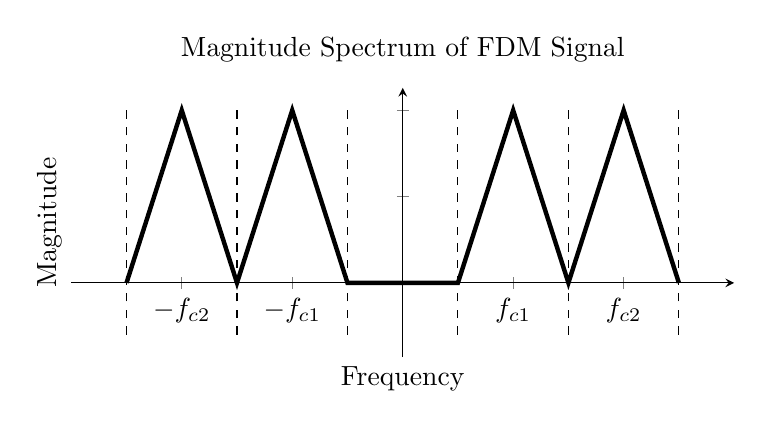
\begin{tikzpicture}
        \begin{axis}[
            title = {Magnitude Spectrum of FDM Signal},
            height = 5cm,
            xlabel = {Frequency},
            ylabel = {Magnitude},
            axis lines = center,
            enlargelimits,
            xtick = {-4, -2, 2, 4},
            xticklabels = {$-f_{c2}$,$-f_{c1}$, $f_{c1}$, $f_{c2}$},
            xticklabel style={fill=white},
            yticklabels = {,,}
            clip=false,
            axis on top,
            x label style={at={(axis description cs:0.5,0)},anchor=north},
            y label style={at={(axis description cs:0,.5)},rotate=90,anchor=south},
            name=ax
            ]
            \addplot[ultra thick, black] coordinates {(-5,0)(-4,1)(-3,0)(-2,1)(-1,0)(1, 0)(2,1)(3,0)(4,1)(5,0)};

            \pgfplotsinvokeforeach{-5,-3,-1,1,3, 5}{
                \addplot [dashed] coordinates {(#1,-0.3)(#1,1)};
            }

        \end{axis}
    \end{tikzpicture}
\end{center}

\noindent
In the case of the habitat's acoustic responses, all intended messages are
multiplexed to occupy 8kHz of bandwidth at differing carrier frequencies. In
order to recover the impulse responses and text messages from the FDM signal,
these different carrier frequencies must be determined, and each signal must be
demodulated.
\subsection*{Spectrum Analyser}
To determine the carrier frequencies for the multiplexed signal, the Fourier
transform of the signal is used to plot the magnitude spectrum in MATLAB. This
is done by first determining the time and frequency vectors for the signal,
knowing that incoming signal is sampled at \verb+fs=576+kHz.

\begin{minted}{matlab}
Ts = 1/fs;                              % Sampling Period [s]
t = 0:Ts:0.5; t(end) = [];              % Time vector
f = linspace(-fs/2, fs/2, length(t)+1); % Frequency Vector
f(end)=[];  
MUXSIG = fft(muxSignal);                % Fourier Transform
\end{minted}

Plotting the signals,

\subsection*{Demultiplexing}
\subsection*{Filtering}
\subsection*{Resampling for Analogue to Digital Conversion}
\subsection*{Resampling for Analogue to Digital Conversion}
\subsection*{Practical Analysis}

\section{Reflection}

\end{document}